\section{Ядро и вектор Шепли. Немного теории.}

Мы ответим на несколько вопросов:

Когда ядро не пусто?

Почему вектор Шепли - это хорошо?

Когда вектор Шепли лежит в ядре?

Поехали!

\subsection{Когда ядро не пусто?}

Разрешим каждому игроку трудиться в нескольких коалициях сразу. Каждый игрок будет распределять свое время (усилия) между теми коалициями, членом которых он является. Причем обяжем всех игроков входящих в одну коалицию трудится в ней одинаковое количество времени. К примеру, в коалиции $S_{1}$ все ее члены трудятся 20\% своего времени, в коалиции $S_{2}$ все ее члены трудятся - 30\% своего времени и т.д. 

С помощью $\lambda_{S}$ обозначим долю своего времени (своих сил), которые тратят на коалицию $S$ ее сотрудники. Конечно же, для любой коалиции $S$ величина $\lambda_{S}\in [0;1]$ и для любого игрока $i$: $\sum_{S, i\in S} \lambda_{S}=1$ (все свои усилия игрок куда-то тратит). 

Для простоты введем:
\begin{mydef}
Набор весов $\lambda_{S}$ называется сбалансированным \index{Сбалансированный набор весов}, если $\forall$ $S$ $\lambda_{S}\in[0;1]$ и $\forall i$ $\sum_{S, i\in S} \lambda_{S}=1$.
\end{mydef}

Критерий непустоты ядра довольно прост:

Большая коалиция должна зарабатывать достаточно много, чтобы суметь пообещать каждой коалиции столько, чтобы у той не было желания отсоединиться. А именно:

Ядро не пусто, если и только если при любом распределении усилий игроков между коалициями их заработок не превосходит заработка большой коалиции.

\begin{myth} $[$Бондарева$]$.\index{Теорема Бондаревой} \index{Критерий непустоты ядра}
Ядро игры в характеристической форме непусто, если и только если для любого сбалансированного набора $\lambda_{S}$:
\begin{equation}
\sum_{S} \lambda_{S}v(S)\leq v(N)
\end{equation}
\end{myth}

\begin{proof}
Если ядро непусто, то существует вектор $x$, такой что: $\sum_{i\in S} x_{i}\geq v(S)$ для любой коалиции $S$, а $  \sum_{i\in N} x_{i}= v(N)$.

Следовательно,
\begin{equation}
\sum_{S} \lambda_{S}v(S) \leq \sum_{S} \lambda_{S} \sum_{i\in S} x_{i} =
\sum_{i}x_{i}\sum_{S, i\in S}\lambda_{S}=\sum_{i}x_{i}\cdot 1=v(N)
%\leq \sum_{S} \lambda_{S} \sum_{i\in N} x_{i} = \sum_{i\in N} x_{i} \sum_{S} \lambda_{S} = \sum_{i\in N} x_{i} \cdot 1 = v(N)
\end{equation}

Доказательство в обратную сторону перенесено в приложение, на стр. \pageref{bond.proof}.
\end{proof}


\subsection{Почему вектор Шепли - это хорошо?}

Когда мы говорили о ядре, мы ввели два хороших свойства (эффективность и отсутствие сепаратистских тенденций), его определяющих. А из этих хороших свойств немедленно следует способ нахождения (решение системы неравенств).

Когда же мы говорили о векторе Шепли, мы ввели способ его подсчета (как матожидание). Потом мы доказали, что он также эффективен. А какими еще хорошими свойствами он обладает?

Давайте поговорим о справедливости! Справедливость для нас будет предcтавлена двумя требованиями: одинаковые игроки должны получать одинаковый выигрыш и бесполезные игроки должны получать ноль.

\begin{mydef}
Назовем игрока <<болваном>> \index{Болван} (dummy player\footnote{В Osborne \cite{osborne:cgt} dummy player определен как игрок, который в каждую коалицию приносит ровно свою стоимость $v(i)$ и ни капли больше. Этому игроку логично выдать $v(i)$ и исключить его из дальнейшего участия в дележе. На меньшее такой игрок не согласен сам, а больше ни одна коалиция не захочет ему платить.}), если он не добавляет ценность ни одной коалции. Игрок $i$ болван, если $\forall S$: $v(S\cup i)=v(S)$. В частности, $v(i)=0$.
\end{mydef}

В соответствии с библейским принципом <<Кто не работает, тот да не ест!>> болваны должны получать ноль.

\begin{mydef} \label{no_bolvans} Платеж удовлетворяет условию <<Болваны получают ноль \index{Болваны получают ноль}>>, если (хм, неожиданно) болваны получают ноль.
\end{mydef}

Например, если в игру <<Носки>> добавить Васю без носков, то было бы справедливо, чтобы ему ничего не доставалось при дележе выигрыша. При подсчете вектора Шепли для игрока болвана $i$ оказывается, что $Add(i,\pi)=0$ для любого порядка $\pi$ и, следовательно, $E(Add(i))=0$.

\begin{mydef} \label{symmetry} Платеж удовлетворяет требованию \indef{симметричности}, \index{требование симметричности} если одинаковые игроки получают одинаковый выигрыш.
\end{mydef}
Если два игрока вносят одинаковый вклад во все коалиции, то хочется, чтобы они получали одинаково. Например, в игре <<Ботинки>> у Лени и у Левы по одному левому ботинку. В векторе Шепли они получают одинаковый выигрыш. Для одинаковых игроков $i$ и $j$ величины их вкладов во все коалиции равны, поэтому случайные величины $Add(i)$ и $Add(j)$ имеют одинаковое распределение. Поэтому и их математические ожидания равны.  

Еще одно требование: линейность. Условия эффективности, симметричности и условие <<болваны получают ноль>> можно сформулировать в рамках одной игры. Условие линейности связывает между собой платежи в разных играх. А именно:
\begin{mydef} \label{linearity}
Правило $f$, которое сопоставляет каждой игре\footnote{Напомним, что для полного описания игры достаточно указать ее характеристическую функцию $v$} $v$ некий дележ $f(v)$, называется \indef{линейным}, если выполнены два условия:

1. $f(c\cdot v)=c\cdot f(v)$

2. $f(v_{1}+v_{2})=f(v_{1})+f(v_{2})$
\end{mydef}

Что это означает? 

Первое требование довольно логично. Пусть есть две игры. Одна задана характеристической функцией $v$. А во второй - выигрыши любой коалиции в $c$ раз больше, чем в первой, т.е. выигрыши задаются функцией $c\cdot v$. Если мы придумали какой-то <<справедливый>> дележ для первой игры, $f(v)$, то <<справедливый>> дележ для второй игры должен быть $c\cdot f(v)$.

Второе требование чуть более трудное. Пусть у нас снова есть две игры, $v_{1}$ и $v_{2}$. Мы придумали правило $f$, которое устанавливает <<справедливый дележ>> для каждой игры, $f(v_{1})$ и $f(v_{2})$. А теперь представим, что наши игроки взаимодействуют между собой два раза. Утром - они играют в игру $v_{1}$, а вечером в игру $v_{2}$. Получилась новая комбинировання игра $v$, которую мы обозначаем как сумму игр, $v=v_{1}+v_{2}$. Естественно, коалиция $S$ работая отдельно от всех утром и вечером заработает $v_{S}=v_{1}(S)+v_{2}(S)$. Согласно второму требованию <<справедливый>> дележ в комбинированной игре, $f(v)$, должен равняться сумме <<справедливых>> дележей в утренней и вечерней играх.

\begin{myth}
Единственным дележом удовлетворяющим требованиям \hyperref[Pareto]{эффективности}, \hyperref[linearity]{линейности}, <<\hyperref[no_bolvans]{болваны получают ноль}>> и \hyperref[symmetry]{симметричности} является вектор Шепли.
\end{myth}

\begin{proof}
Мы уже фактически доказали, что вектор Шепли удовлетворяет требованиям эффективности, симметричности и требованию <<болваны получают ноль>>. 

Линейность. Одновременно рассмотрим три кооперативных игры: $v_{1}$, $v_{2}$ и комбинированную игру $v=v_{1}+v_{2}$. Есть некий порядок $ \pi $ формирования большой коалиции. Пусть до входа игрока $i$ уже сформирована коалиция $S$. Добавка $Add_{v}(i,pi)$ в комбинированной игре является суммой добавок в утренней и вечерней играх:
\begin{equation}
Add_{v}(i,pi)=Add_{v_{1}}(i,pi)+Add_{v_{2}}(i,pi)
\end{equation}

Т.к. это верно для любого порядка $ \pi $ формирования большой коалиции, получается, что вклад $ i $-го игрока в комбинированной игре (как случайная величина) распадается в аналогичную сумму: $Add_{v}(i)=Add_{v_{1}}(i)+Add_{v_{2}}(i)$. Берем математическое ожидание: $E(Add_{v}(i))=E(Add_{v_{1}}(i))+E(Add_{v_{2}}(i))$. И получаем линейность вектора Шепли: $\phi_{i}(v)=\phi_{i}(v_{1})+\phi_{i}(v_{2})$.

То, что вектор Шепли удовлетворяет первому свойству: $\phi_{i}(cv)=c\phi_{i}(v)$ - аналогично следует из того, что константу можно выносить за знак математического ожидания.

Пусть теперь какое-нибудь правило дележа удовлетворяет четырем требованиям. Докажем, что это может быть только вектор Шепли.
Для начала докажем это для простых игр.

\begin{mydef}
Игра в характеристической форме называется \indef{простой}\index{Простая игра}, если существует особая коалиция $S$, такая что без ее участия в полном составе нельзя получить ничего, а с ее участием в полном составе можно получить единицу:

\begin{equation}
v(K):=
\begin{cases} 
1, S\subset K \\  
0, S\not \subset K \\
\end{cases}
\end{equation}

\end{mydef}

Иногда простые игры называют олигархическими, а игроков, входящих в особую коалицию $S$ - олигархами\index{Олигархическая игра}.

Поскольку в простой игре все игроки не входящие в $S$ - болваны\footnote{Да, каждый игрок либо олигарх, либо болван.}, то они получают 0 (условие <<болваны получают ноль>>). А игроки входящие в $S$ неразличимы между собой, и поэтому обязаны делить общий заработок $v(N)=1$ поровну (условие эффективности плюс условие симметричности), т.е. получать $\frac{1}{|S|}$.
Значит, для простых игр условия <<болваны получают ноль>>, симметричность и эффективность однозначно определяют дележ. А вектор Шепли им всегда удовлетворяет. Значит в простых играх вектор Шепли - единственное условие удовлетворяющее указанным требованиям.

Рассмотрим произвольную игру в характеристической форме. Она полностью определяется функцией $v$. Функцию $v$ можно записать в виде $v=\sum_{S}\mu(S)v_{S}$, где $v_{S}$ это игра с олигархической коалицией $S$, а $\mu_{S}$ - некоторые коэффициенты. Это не что иное, как разложение вектора с помощью базиса. Оно единственно, но нам даже этот факт не нужен. Для наглядности лишь приведем пример:

\begin{myex}
Разложение игры <<Носки>> на простые игры. $v=60v_{\mbox{Андрей}}+120v_{\mbox{Борис}}+60v_{\mbox{Андрей, Борис}}$.
\end{myex}


Для простых игр существует единственный дележ удовлетворяющий трем условиям (эффективность, симметричность, <<болваны получают ноль>>). Характеристическая функция любой игры получается как линейная комбинация характеристических функций простых игр, значит если от дележа дополнительно потребовать линейность, то дележ получается единственным в любой игре.
\end{proof}

\subsection{Когда вектор Шепли лежит в ядре?}

Есть такой красивое словосочетание <<эффект снежного кома>>. Каков его смысл? Если катить маленький снежок, то он медленно растет, а если катить большой ком снега, то он быстро растет. Эта идея иногда верна и в кооперативных играх. К примеру, Вовочка подбивает Петю бойкотировать контрольную, которую устравивает Марь Иванна. Если бойкотировать контрольную пока согласен только сам Вовочка, то Петя мало что добавит к выигрышу Вовочки. А если бойкотировать уже согласны все в классе кроме Пети, то присоединение Пети к бойкотирующим резко увеличивает их выигрыш.

Возникает следующее определение.
\begin{mydef}
Игра в характеристической форме проявляет <<эффект снежного кома\index{Эффект снежного кома}>> (snowball effect), если для любого игрока $i$ и для любых коалиций $K\subset L$ не содержащих игрока $i$ выполнено условие:
\begin{equation}
v(K\cup i)-v(K)\leq v(L\cup i)-v(L)
\end{equation}
\end{mydef}

Левая часть неравенства - это выигрыш маленькой коалиции $K$ от присоединения Пети, а правая часть - выигрыш крупной коалиции $L$ от присоединения Пети.

Это определение эквивалентно более общепринятому, но менее наглядному определению супермодулярности:
\begin{mydef}
Игра в характеристической форме называется супермодулярной \index{Супермодулярность}\index{Супермодулярная игра} (supermodular или convex\footnote{Слово convex оказывается слишком перегруженным (есть convex set, convex function и пр.), поэтому чтобы избежать путаницы лучше использовать supermodular.}), если для любых коалиций $S$ и $T$:
\begin{equation}
v(S\cup T)+v(S\cap T)\geq v(S)+v(T)
\end{equation}
\end{mydef}

Докажем эквивалентность определений:
\begin{proof}
Пусть игра $v$ - супермодулярна. Пусть $K\subset L$, $i\notin L$. Рассмотрим коалиции $S=(K,i)$ и $T=L$. Применяем супермодулярность:
\begin{equation}
v((K,i)\cup L)+v((K,i)\cap L)\geq v(K,i)+v(L)
\end{equation}
Игрок $i$ не лежит ни в $K$, ни в $L$, поэтому:
\begin{equation}
v(L,i)+v(K)\geq v(K,i)+v(L)
\end{equation}
Что дает определение игры с эффектом снежного кома.

Пусть игра $v$ обладает эффектом снежного кома. Пусть $S$ и $T$ - две произвольные коалиции. 

Шаг 1. Рассмотрим коалиции $K=S\cap T$ и $L=T$. По определению $K\subset L$. Рассмотрим произвольного игрока, $i\in S\backslash T$.
В силу эффекта снежного кома:
\begin{equation}
v(K\cup i)-v(K)\leq v(L\cup i)-v(L)
\end{equation}

Шаг 2. Добавим в коалиции $K$ и $L$ игрока $i$, при этом конечно, $(K,i)\subset (L,i)$. Рассмотрим нового произвольного игрока, $j\in S\backslash T$, $j\neq i$. Применяем эффект снежного кома к $(K,i)\subset (L,i)$:
\begin{equation}
v((K,i)\cup j)-v(K,i)\leq v((L,i)\cup j)-v(L,i)
\end{equation}

Заметьте, что если сложить эти два неравенства, то получится:
\begin{equation}
v(K,i,j)-v(K)\leq v(L,i,j)-v(L)
\end{equation}
Это легко интерпретируется: если два игрока $i$ и $j$ вступают в более крупную коалицию $L\supset K$, то они приносят больший доход.

Продолжая добавлять по одному игроков из $S\backslash T$ и складывая неравенства мы получим, что:
\begin{equation}
v(K\cup (S\backslash T))-v(K)\leq v(L\cup (S\backslash T))-v(L)
\end{equation}
Вспомнив, что $K=S\cap T$, а $L=T$, получаем:
\begin{equation}
v(S)-v(S\cap T)\leq v(T\cup S)-v(T)
\end{equation}
что является определением супермодулярности.
\end{proof}

Игры с <<эффектом снежного кома>> хороши тем, что:

\begin{myth}
Ядро супермодулярной игры непусто
\end{myth}
\begin{proof}

Зафиксируем произвольный порядок формирования большой коалиции $\pi$. Оказывается, что вектор $(Add(1,\pi),Add(2,\pi),....,Add(n,\pi))$ лежит в ядре. Действительно:

Для того, чтобы не перегружать доказательство индексами поступим так. Во-первых, поскольку нумерация игроков произвольна, будем считать, что игроки входят в порядке: 1,2,3..., $n$. Если они входят в другом порядке, то перенумеруем их. Во-вторых, введем обозначение $K_{i}$ - это первые $i$ игроков, $K_{i}=\{1,2,3,...,i\}$. До игрока $i$, естественно успели войти игроки из $K_{i-1}$.

Шаг 1. Рассмотрим произвольную коалицию из одного игрока $i$.

В силу супермодулярности: 
\begin{equation}
v(K_{i-1}\cap i)+v(K_{i-1}\cup i)\geq v(K_{i-1})+v(i) 
\end{equation}

Что равносильно: 

\begin{equation}
v(i)\leq v(K_{i-1}\cup i)-v(K_{i-1})
\end{equation}

Значит, $v(i)\leq Add(i,\pi)$.
Итак, ни один игрок не выиграет, если откажется от предлагаемого дележа и возьмет $v(i)$.

Индукция. Допустим мы доказали, что ни одной коалиции из $k-1$ игрока не выгодно отсоединятся. Рассмотрим произвольную коалицию $K$ из $k$ игроков. В этой коалиции есть игрок с наибольшим номером $m$. Значит $K\subset K_{m}$, но $K\not \subset K_{m-1}$. 

В силу супермодулярности:
\begin{equation}
v(K_{m-1}\cap K)+v(K_{m-1}\cup K)\geq v(K_{m-1})+v(K) 
\end{equation}

Заметив, что $K_{m-1}\cup K=K_{m}$ получаем:

\begin{equation}
v(K_{m-1}\cap K)+v(K_{m})-v(K_{m-1})\geq v(K) 
\end{equation}

Разница $v(K_{m})-v(K_{m-1})$ - это то, что вектор Шепли отдает $m$-му игроку, т.е. $v(K_{m})-v(K_{m-1})=Add(m,\pi)$.

В коалиции $K_{m-1}\cap K$ меньше участников, чем в $K$, значит по предположению индукции ей не выгодно отсоединяться, т.е.
\begin{equation}
\sum_{i\in K_{m-1}\cap K}Add(i,\pi)\geq v(K_{m-1}\cap K)
\end{equation}

Получаем, что:
\begin{equation}
\sum_{i\in K_{m-1}\cap K}Add(i,\pi) + Add(m,\pi)\geq v(K)
\end{equation}

Но в левой части стоит ровно та сумма денег, которая предлагается коалиции $K$, а значит и ей не выгодно отсоединятся.
\end{proof}

Поскольку векторы $(Add(1,\pi),Add(2,\pi),....,Add(N,\pi))$ - это то, что усредняет вектор Шепли мы немедленно получаем:


\begin{myth}
Если игра - супермодулярная, то вектор Шепли лежит в ядре
\end{myth}
\begin{proof}
Ядро задается системой линейных неравенств, значит оно является выпуклым множеством. 

Поскольку для любого фиксированного порядка формирования большой коалиции $\pi$ вектор 
\begin{equation}
(Add(1,\pi),Add(2,\pi),....,Add(N,\pi))
\end{equation}
лежит в ядре, то и весь многогранник, что находится <<между>> этими векторами лежит в ядре. Значит и вектор Шепли, как среднее арифметическое этих векторов-вершин многогранника, также лежит в ядре.
\end{proof}

Более того, в супермодулярных играх ничего кроме этого многогранника в ядро и не входит.

\begin{myth}
Ядро супермодулярной игры - это многогранник \index{Многогранник} с вершинами в $(Add(1,\pi),Add(2,\pi),....,Add(n,\pi))$, где $\pi$ - это всемозвожные порядки формирования большой коалиции.
\end{myth}

Оставим это утверждение без доказательства, но проиллюстрируем. 

Возьмем для примера игру, где Алеша Попович, Добрыня Никитич и Илья Муромец ловят драконов. В одиночку - никто не может поймать, вдвоем они ловят $\alpha$ драконов в час, втроем - одного дракона в час. Если мы формируем коалицию в случайном порядке, то первый входящий получает ноль, второй - $\alpha$, а вклад третьего - $(1-\alpha)$. Соответственно наш многогранник (в данном случае все грани оказались в одной плоскости, так вышло) имеет 6 вершин. Шесть вершин - это векторы из чисел 0, $\alpha$ и $(1-\alpha)$ во всех возможных порядках.


\begin{figure}[htbp]
   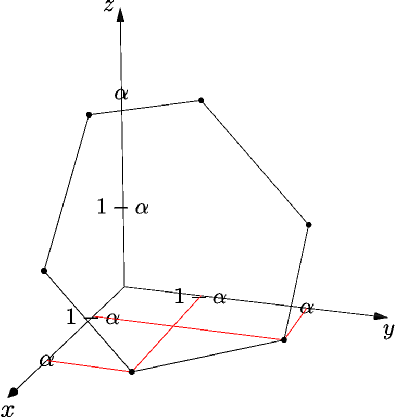
\includegraphics{coop_3player.pdf}
\end{figure}




\subsection{Окончание доказательства т. Бондаревой, критерия непустоты ядра}

Напомним формулировку:
\begin{myth} $[$Бондарева$]$.
Ядро игры в характеристической форме непусто, если и только если для любого сбалансированного набора $\lambda_{S}$:
\begin{equation}
\label{balanced_game2}
\sum_{S} \lambda_{S}v(S)\leq v(N)
\end{equation}
\end{myth}

\begin{proof} \label{bond.proof}

Обратно\footnote{Приведенное доказательство взято из Osborne, Rubinstein, \cite{osborne:cgt}. У Данилова в \cite{danilov:lte} через т. Какутани. Может есть еще более геометрическое доказательство?}. Пусть неравенство \ref{balanced_game2} выполнено.

Для доказательства в обратную сторону нам понадобится технических факт:
\begin{myth}
Два выпуклых множества в $R^{n}$ можно разделить гиперплоскостью. Более алгебраическая формулировка: если есть два выпуклых непересекающихся множества, $A$ и $B$, то существует вектор $\vec{\alpha}$ и число $c$, такие, что для любых $a\in A$ и $b\in B$ верно неравенство: $\vec{\alpha}\cdot b \geq c \geq \vec{\alpha}\cdot a$.
\end{myth}
Этот факт мы примем без доказательства как хорошо согласующийся с геометрическими представлениями.

[Картинка <<и ежу понятно>>]
\begin{figure}[htbp]
	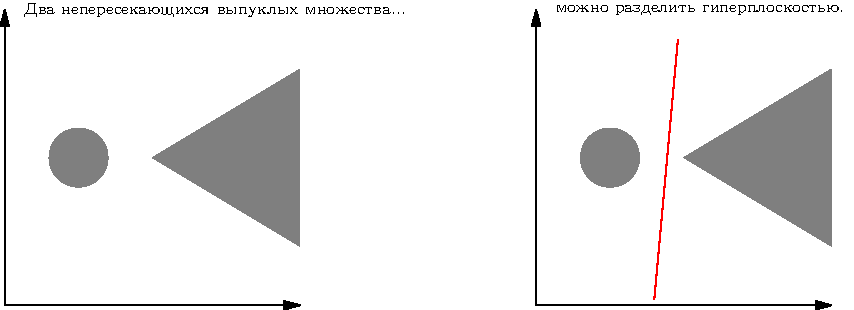
\includegraphics{coop_separating.pdf}
\end{figure}


Введем обозначение $1_{S}$ - это вектор из $n$ чисел, каждое из которых равно нулю или единице, в зависимости от того, входит ли соответствующий участник в коалицию $S$. В частности, $1_{N}$ - это вектор из $n$ единичек, а $1_{\emptyset}$ - это вектор из $n$ нулей. Например, если $N=\{A,B,C,D\}$ и коалиция $S=\{A,D\}$, то $1_{S}=(1,0,0,1)$. Убедитесь, что на этом языке условие сбалансированности набора весов записывается как
\begin{equation}
\sum_{S} \lambda_{S}1_{S}=1_{N}
\end{equation}

Вектор $1_{S}$ лежит в $n$-мерном пространстве.

Допишем к вектору $1_{S}$ стоимость соответствующей коалиции, получим вектор $(1_{S},v(S))$, лежащий в $(N+1)$-мерном пространстве.

Рассмотрим два множества (в $R^{n+1}$):

$A=\{(1_{N},v(N)+\varepsilon)| \varepsilon>0\}$. Это множество выпуклое, т.к. это полупрямая с выколотым началом.

$B=\{\sum_{S} \lambda_{S} (1_{S},v(S)) | \forall  \lambda_{S}\geq 0 \}$. Это множество также выпуклое, т.к. это конус (пирамида). Вершина этого конуса - начало координат. Образующие - векторы вида $(1_{S},v(S))$.


Эти множества не имеют общих точек, в силу неравенства \ref{balanced_game2}. Заметим, что если бы в множестве $A$ была бы разрешена точка c $\varepsilon=0$, т.е. точка $(1_{N},v(N))$, то она и была бы общей.

Для наглядности приведем график\footnote{На самом деле там есть 3d модель, но pdftex из комплекта texlive похоже не может ее присоединить, поэтому пока есть только ее проекция. Если кто знает, как это исправить - напишите.} для двух игроков. Вертикальная ось будет отвечать за $v(S)$. А две остальные оси - за первого и второго игрока. 

\begin{figure}[htbp]
	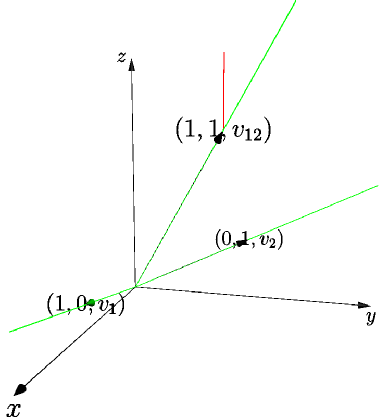
\includegraphics{coop_bondar.pdf}
\end{figure}

Конус с образующими $(1,0,v_{1})$, $(0,1,v_{2})$ и $(1,1,v_{12})$ - это множество $B$, а полупрямая стартующая <<вверх>> из точки $(1_{N},v(N))$ на конусе - это множество $A$. 

 Оба множества выпуклы, значит существует гиперплоскость разделяющая множества $A$ и $B$. Эта гиперплоскость, конечно же проходит через точку $(1_{N},v(N))$. Из рисунка ясно, что можно взять гиперплоскость, содержащую образующую конуса $(1_{N},v(N))$. Т.е. разделяющая гиперплоскость проходит через начало координат. Здесь мы неявно воспользовались супераддитивностью, т.к. нам надо, чтобы образующая $(1_{N},v(N))$ лежала <<выше>> остальных образующих.


В общем случае гиперплоскость определяется ненулевым вектором $\vec{\alpha}=(\alpha_{1},\alpha_{2},...,\alpha_{n+1})$ и числом $c$ так что:

\begin{equation}
	\vec{\alpha}\cdot b \geq c \geq \vec{\alpha}\cdot a
\end{equation},
для любых $a\in A$ и $b\in B$.

В нашем случае есть два уточнения. Поскольку множество $A$ открытое, то правое неравенство можно заменить на строгое.
А поскольку гиперплоскость проходит через начало координат, то константа $c$ равна 0.

Значит применительно к нашему случаю существование разделяющей гиперплоскости выглядит так:

\begin{equation}
\label{hyperplane_eq}
	\vec{\alpha}\cdot b \geq 0 > \vec{\alpha}\cdot a
\end{equation},
для любых $a\in A$ и $b\in B$.


Сначала мы заметим, что $\alpha_{n+1}<0$, а затем построим из $(\alpha_{1},\alpha_{2},...,\alpha_{n})$ элемент ядра.

Разделяющая гиперплоскость проходит через начало координат. Верхняя часть вертикальной оси, т.е. множество $\{(0,...,0,v)|v>0\}$ лежит в той же половине пространства, что и множество $A$. Значит $\alpha_{n+1}\cdot v<0$. Значит $\alpha_{n+1}<0$.

%Заметим, что $\alpha_{n+1}$ не может быть положительным: если бы оно было положительным можно было бы взять вектор $a$ с большим $\varepsilon$ и добиться положительности $\vec{\alpha}\cdot a$.

%Уточним, что $\alpha_{n+1}$ не может быть равен нулю. Для этого рассмотрим вектор $v=(1_{N},v(N))$, начало полупрямой $A$. Он лежит в множестве $B$ - достаточно взять $\lambda_{N}=1$, а остальные $\lambda_{S}=0$. Поскольку вектор $v$ попадает на границу $A$ для него неравенство выглядит так: $\vec{\alpha}\cdot v \geq 0 \geq \vec{\alpha}\cdot v$.

%Заметим, что $\vec{\alpha}\cdot v=\sum_{i=1}^{N}\alpha_{i}+\alpha_{n+1}v(N)$.

%При $\alpha_{n+1}$ равном нулю мы получали бы, что $\sum_{i=1}^{n}\alpha_{i}=0$. Но это невозможно, т.к. в этом случае $\vec{\alpha}\cdot a$ равнялось бы нулю.

Поделим неравенство \ref{hyperplane_eq} на $(-\alpha_{n+1})$. При этом знаки неравенства не поменяются, а последняя компонента вектора $\vec{\alpha}$ превратится в минус единицу. Обозначим: $x_{i}=-\alpha_{i}/\alpha_{n+1}$.

Что это нам дает?

Левая часть неравенства говорит: для любого $b$: $(x_{1},x_{2},...,x_{n},-1)\cdot b \geq 0$.

Возьмем $b=(1_{S},v(S))$. Получаем, $\sum_{i\in S}x_{i}\geq v(S)$.

Правая часть неравенства говорит: для любого $a$: $(x_{1},x_{2},...,x_{n},-1)\cdot a <0$.

Возьмем $v=(1_{N},v(N))$. Этот вектор в $A$ не входит, но лежит на границе $A$, поэтому неравенство будет нестрогим: $\sum_{i\in N}x_{i}\leq v(N)$.

Что это значит? Это означает, что есть такой вектор $x$, который большая коалиция может выплатить (может у нее даже что-то останется). При этом ни одна коалиция $S$ не может получить больше, чем достается ей при дележе $x$. Следовательно, ядро не пусто.

\end{proof}
